\documentclass{article}
\usepackage[utf8]{inputenc}
\usepackage[english]{babel}
\usepackage{amssymb}
\usepackage{amsmath}
\usepackage{graphicx}

\usepackage{geometry}
\geometry{left=2.5cm,right=2.5cm,top=2cm,bottom=2cm}

\setlength{\parskip}{0.5em}
\setlength{\parindent}{0em}
\renewcommand{\baselinestretch}{1.0}

\title{Assignment 1}
\author{COL 352\\
    Introduction to Automata \& 
    Theory of Computation}
\date{}

\begin{document}

\maketitle

\section*{Problem 1}

\textbf{1.1.} 
$L = (0|1)^{*}(101)(0|1)^{*}$\\
The NFA represents the language which contains 101 as a substring 

\textbf{1.2.}
$L = (0|1)^{*}$\\
The NFA accepts all the strings defined over the alphabet $\sum = (0|1)$

\textbf{1.3.}
Complementing the states of NFA does not necessarily complement the language accepted by the original NFA. However, the above claim is true for a Deterministic Finite State Automata. 


\section*{Problem 2}
Following is the DFA for 

$L = \{ w \in  \{0, 1\}^{*} | w$ contains the substring 110 or 0001\} where \\
$Q = \{A, B, C, D, E, F\} \\
\sum = \{0 , 1\} \\
q_{0} = A \\
F = \{ G \}$

\begin{figure}[h]
\centering
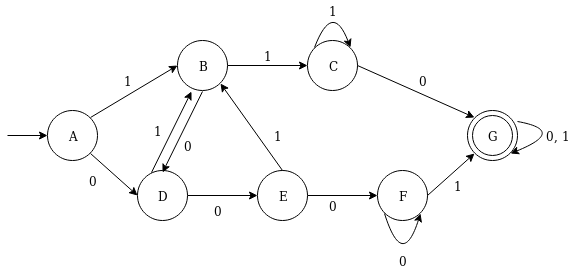
\includegraphics[scale=0.5]
{Images/q1.png}
\caption{DFA for \textit{L}}
\end{figure} 


A: starting state \\
B: indicates '1' or '01' has been encountered, i.e, one '1' has been encountered \\
C: indicates '11' has been encountered \\
D: indicates '0' or '10' has been encountered, i.e, one '0' has been encountered \\
E: indicates '00' has been encountered \\
F: indicates '000' has been encountered \\
G: indicates either '110' or '0001' has been encountered and thus a final state

Thus this DFA accepts only $L$
\end{document}